\documentclass[aspectratio=169,10pt]{beamer}
\usepackage[UTF8,fontset=fandol]{ctex}
\usepackage{amsmath,amssymb,booktabs,array,multirow}
\usepackage{graphicx,xcolor,tikz}
\usetikzlibrary{arrows.meta,positioning,fit,calc,shapes.geometric}
\usepackage{hyperref}

\definecolor{DeepBlue}{HTML}{17365D}
\definecolor{Ocean}{HTML}{2878B5}
\definecolor{Teal}{HTML}{1B998B}
\definecolor{Orange}{HTML}{F28E2B}
\definecolor{Red}{HTML}{D9534F}
\definecolor{Green}{HTML}{3A923A}
\definecolor{LightBlue}{HTML}{EAF3F8}
\usetheme{Madrid}
\setbeamercolor{structure}{fg=DeepBlue}
\setbeamercolor{frametitle}{fg=white,bg=DeepBlue}
\setbeamercolor{title}{fg=white}
\setbeamercolor{titlelike}{bg=DeepBlue}
\setbeamercolor{block title}{fg=white,bg=Ocean}
\setbeamercolor{block body}{bg=LightBlue}
\setbeamercolor{alerted text}{fg=Red}
\setbeamertemplate{navigation symbols}{}
\setbeamertemplate{footline}{\leavevmode\hbox{%
  \begin{beamercolorbox}[wd=.82\paperwidth,ht=2.6ex,dp=1.1ex,leftskip=1em]{author in head/foot}\color{DeepBlue}\insertshorttitle\end{beamercolorbox}%
  \begin{beamercolorbox}[wd=.18\paperwidth,ht=2.6ex,dp=1.1ex,center]{date in head/foot}\color{DeepBlue}\insertframenumber/\inserttotalframenumber\end{beamercolorbox}}}
\setlength{\tabcolsep}{4pt}
\newcommand{\code}[1]{\texttt{#1}}
\newcommand{\videotext}[2]{\href{run:./media/#1}{\textcolor{Ocean}{\underline{#2}}}}

\title[分层视觉落足控制]{分层视觉落足控制框架：方法实现与阶段结果}
\subtitle{下层闭环落足执行器与上层潜空间预测控制}
\author{Mind-Steps / Upper Foothold Planner 项目总结}
\date{2026 年 8 月 25 日}

\begin{document}

\begin{frame}
  \titlepage
\end{frame}

\begin{frame}{报告内容与当前完成状态}
\begin{columns}[T,onlytextwidth]
\column{0.55\textwidth}
\begin{block}{方法构成}
\begin{enumerate}
  \item 下层：根据左右脚目标位姿与步态相位，50 Hz 输出 8 维关节位置增量；
  \item 上层：根据深度图、本体状态与导航目标，每次换脚规划一个三维落足动作；
  \item 连接：上层动作被解码为世界坐标脚目标，再由冻结下层闭环执行。
\end{enumerate}
\end{block}
\column{0.42\textwidth}
\begin{block}{已完成的验证}
\begin{itemize}
  \item 下层连续 50 s、99 次触地；
  \item 单障碍视觉闭环绕行；
  \item 三障碍多步预测对照；
  \item 窄桥落足规划对照；
  \item 典型地形运行与失败案例。
\end{itemize}
\end{block}
\end{columns}
\vspace{0.3em}
本报告聚焦\textbf{可复现的方法定义、代码实现和已有结果}；候选应用仅保留为方法提案，不展开论文包装与大规模对比计划。
\end{frame}

\begin{frame}{总体架构：两个时间尺度的闭环控制}
\centering
\begin{tikzpicture}[node distance=6mm and 8mm,>=Latex,every node/.style={font=\small,align=center}]
\node[draw,rounded corners,fill=LightBlue,minimum width=30mm,minimum height=12mm] (sensor) {深度图 $D_k$\; 本体 $p_k$\;目标 $g_k$};
\node[draw,rounded corners,fill=orange!15,right=of sensor,minimum width=32mm,minimum height=12mm] (upper) {上层世界模型+CEM\\$u_k=(\rho_k,\theta_k,\psi_k)$};
\node[draw,rounded corners,fill=green!15,right=of upper,minimum width=30mm,minimum height=12mm] (decode) {落足目标解码\\$T_k^L,T_k^R$};
\node[draw,rounded corners,fill=blue!10,below=11mm of upper,minimum width=38mm,minimum height=12mm] (lower) {冻结下层 Actor\\$a_t=\pi_\ell(o_t,c_t)$};
\node[draw,rounded corners,fill=gray!15,left=of lower,minimum width=30mm,minimum height=12mm] (pd) {PD 控制与机器人\\$\tau_t$};
\draw[->,thick] (sensor)--(upper);
\draw[->,thick] (upper)--(decode);
\draw[->,thick] (decode)--(lower);
\draw[->,thick] (lower)--(pd);
\draw[->,thick] (pd.west) -- ++(-8mm,0) |- (sensor.south);
\end{tikzpicture}
\vspace{0.8em}
\begin{tabular}{lll}
\toprule
层级 & 更新时刻 & 作用对象\\
\midrule
下层 $t$ & $\Delta t_\ell=0.02$ s（50 Hz） & 8 个关节位置目标\\
上层 $k$ & $\Delta t_h=0.5$ s（一次换脚，25 个下层步） & 下一步距离、方向和脚偏航\\
\bottomrule
\end{tabular}
\end{frame}

\begin{frame}{符号、坐标系与上下层接口}
\small
\begin{tabular}{p{0.13\textwidth}p{0.80\textwidth}}
\toprule
符号 & 含义\\
\midrule
$W,B,F_s$ & 世界坐标系、机身坐标系、当前支撑脚坐标系\\
$p^A_X,q^A_X$ & 对象 $X$ 在坐标系 $A$ 下的位置与四元数；四元数内部顺序为 $wxyz$\\
$L,R,s,w$ & 左脚、右脚、支撑脚和摆动脚索引\\
$t,k$ & 下层控制步与上层宏观步；一个 $k$ 通常覆盖 25 个 $t$\\
$T^i_k=(p^W_{i,*},q^W_{i,*})$ & 上层给脚 $i\in\{L,R\}$ 的目标位姿\\
$c_t\in\mathbb{R}^{16}$ & 下层目标编码；由两脚相对目标与步态相位组成\\
$o_t^\pi,o_t^V$ & 下层 Actor 与 Critic 的原始观测，维数分别为 30、33\\
$D_k,p_k,g_k$ & 上层深度图、本体向量和相对导航目标\\
$u_k=(\rho_k,\theta_k,\psi_k)$ & 上层动作：步长、支撑脚局部方向、目标脚偏航增量\\
\bottomrule
\end{tabular}
\vspace{0.5em}
所有上层位移动作都在 $F_s$ 的水平朝向坐标系中定义，因此同一个 $u_k$ 可直接迁移到不同世界位置和机器人朝向。
\end{frame}

\begin{frame}{下层任务定义：闭环执行左右脚目标位姿}
\begin{columns}[T,onlytextwidth]
\column{0.56\textwidth}
在每个下层时刻 $t$，策略为
\[
 a_t\sim\pi_\ell(a\mid \hat o_t^\pi,\hat c_t),\qquad a_t\in[-1,1]^8 .
\]
其中：
\begin{itemize}
  \item $a_t$：8 个关节的位置增量；
  \item $\hat o_t^\pi$：归一化后的 Actor 本体观测；
  \item $\hat c_t$：归一化后的双脚目标编码；
  \item $\pi_\ell$：随机高斯策略，执行时取均值。
\end{itemize}
关节目标和力矩为
\[
q_t^d=\operatorname{clip}(q^0+a_t,q^{\min},q^{\max}),
\]
\[
\tau_t=\operatorname{clip}\!\left(K_p(q_t^d-q_t)-K_d\dot q_t,-80,80\right).
\]
\column{0.41\textwidth}
\begin{block}{控制器参数}
\begin{itemize}
  \item $q^0$：默认关节角；
  \item $q_t,\dot q_t$：当前关节角、角速度；
  \item $q^{\min},q^{\max}$：关节限位；
  \item $K_p=45$；
  \item 踝关节 $K_d=0.8$，其余 $K_d=1.5$；
  \item 力矩上限 $80$ N$\cdot$m；
  \item 物理步长 0.005 s，控制降采样 4。
\end{itemize}
\end{block}
\end{columns}
\end{frame}

\begin{frame}{下层 Actor/Critic 输入：维度与排列顺序}
\scriptsize
\begin{columns}[T,onlytextwidth]
\column{0.49\textwidth}
\begin{block}{Actor 原始本体观测 $o_t^\pi\in\mathbb{R}^{30}$}
\begin{tabular}{lr}
\toprule
字段（按代码拼接顺序）& 维数\\
\midrule
机身坐标重力向量 $\bar g_t$ & 3\\
关节角 $q_t$ & 8\\
世界坐标机身角速度 $\omega_t$ & 3\\
$0.1\dot q_t$ & 8\\
上一步策略动作 $a_{t-1}$ & 8\\
\midrule
合计 & 30\\
\bottomrule
\end{tabular}
\end{block}
Actor 实际输入为 $[\hat o_t^\pi,\hat c_t]\in\mathbb{R}^{46}$。
\column{0.49\textwidth}
\begin{block}{Critic 原始观测 $o_t^V\in\mathbb{R}^{33}$}
\begin{tabular}{lr}
\toprule
字段（按代码拼接顺序）& 维数\\
\midrule
机身坐标重力向量 $\bar g_t$ & 3\\
关节角 $q_t$ & 8\\
世界坐标机身线速度 $v_t$ & 3\\
世界坐标机身角速度 $\omega_t$ & 3\\
关节角速度 $\dot q_t$ & 8\\
上一步策略动作 $a_{t-1}$ & 8\\
\midrule
合计 & 33\\
\bottomrule
\end{tabular}
\end{block}
Critic 实际输入为 $[\hat o_t^V,\hat c_t]\in\mathbb{R}^{49}$；Actor 不使用机身线速度，Critic 训练时可使用。
\end{columns}
\vspace{0.4em}
本体观测、目标编码和 Critic 观测分别用运行均值方差归一化，并截断到 $[-10,10]$。
\end{frame}

\begin{frame}{下层目标编码：支撑脚相对的 16 维表示}
\small
对脚 $i\in\{L,R\}$，把世界目标 $T^i=(p^W_{i,*},q^W_{i,*})$ 表示到当前支撑脚 $F_s$：
\[
\Delta p_i=R(q^W_s)^\top(p^W_{i,*}-p^W_s)\in\mathbb{R}^3,
\qquad
\Delta q_i=(q^W_s)^{-1}\otimes q^W_{i,*}\in\mathbb{H}.
\]
若 $\Delta q_i$ 的实部为负，则整体乘 $-1$，消除 $q$ 与 $-q$ 的双覆盖。最终编码为
\[
c_t=[\Delta p_L,\Delta q_L,\Delta p_R,\Delta q_R,
\cos(2\pi\phi_t),\sin(2\pi\phi_t)]\in\mathbb{R}^{16}.
\]
\begin{itemize}
  \item $R(q)$：四元数 $q$ 对应的旋转矩阵；$\otimes$：四元数乘法；
  \item $p^W_s,q^W_s$：当前支撑脚世界位姿；$p^W_{i,*},q^W_{i,*}$：脚 $i$ 的目标位姿；
  \item $\Delta p_i,\Delta q_i$：目标相对支撑脚的位置和姿态；
  \item $\phi_t\in[0,1)$：1 Hz 步态相位，$[0,0.5)$ 左脚摆动，$[0.5,1)$ 右脚摆动。
\end{itemize}
支撑脚目标在相位切换时锁存，摆动脚目标持续作为闭环参考。
\end{frame}

\begin{frame}{下层目标采样器：训练分布的完整定义}
\scriptsize
每次需要新摆动目标时，采样步长 $d$、方向扰动 $\alpha$ 和脚偏航扰动 $\beta$：
\[
d\sim\mathcal U(0.07,d_{\max}),\quad \alpha\sim\mathcal U(-30^\circ,30^\circ),
\quad\beta\sim\mathcal U(-30^\circ,30^\circ),
\]
\[
p^W_{w,*}=p^W_s+d[\cos(\chi+\alpha),\sin(\chi+\alpha),0]^\top,
\quad \psi^W_{w,*}=\psi_s+\beta.
\]
\begin{tabular}{p{0.23\textwidth}p{0.69\textwidth}}
\toprule
符号/规则 & 定义\\
\midrule
$d_{\max}$ & 前 500 次迭代由 0.15 m 线性增至 0.35 m\\
$\chi$ & 每回合采样的运动朝向，范围 $[-180^\circ,180^\circ]$\\
$p^W_{w,*},\psi^W_{w,*}$ & 新摆动脚的世界目标位置与偏航角\\
防交叉约束 & 转到支撑脚偏航坐标后，左脚横向 $y\ge0.10$ m、右脚 $y\le-0.10$ m\\
最小变化 & 候选目标距当前摆动脚小于 0.05 m 时重采样，最多 10 次\\
原地保持 & 概率 0.10；每 10 个步态周期重采样；保持阈值 0.20 m\\
朝向限制 & 相对支撑脚偏航截断在 $[-90^\circ,90^\circ]$\\
\bottomrule
\end{tabular}
\vspace{0.3em}
该采样器既产生多方向落足能力，也明确限定了下层可执行动作域，上层动作范围必须落在该域内。
\end{frame}

\begin{frame}{下层奖励：统一形式与跟踪项}
\scriptsize
每个控制步的总奖励为
\[
r_t=\Delta t_\ell\sum_m w_m\,\varrho_m(t),\qquad \Delta t_\ell=0.02\ \mathrm{s},
\]
其中 $m$ 为奖励项索引，$w_m$ 为权重，$\varrho_m$ 为未加权奖励。跟踪核心为：
\begin{align*}
\varrho_{xy}&=\exp(-100\|p^{xy}_{w,t}-p^{xy}_{w,*}\|_2^2), &w_{xy}=5,\\
\varrho_z&=\exp[-100(p^z_{w,t}-z^d_t)^2], &w_z=4,\\
\varrho_\psi&=\exp[-100\,e_\psi(q^W_{w,t},q^W_{w,*})^2], &w_\psi=0.4,\\
\varrho_h&=\exp[-100\,\delta h_t^2\,\eta(\phi_t)](1-I_{\rm hold}), &w_h=4.
\end{align*}
\begin{itemize}
  \item $p_{w,t},q^W_{w,t}$：摆动脚当前位姿；$p_{w,*},q^W_{w,*}$：目标位姿；$e_\psi$：包裹到 $[-\pi,\pi]$ 的偏航误差；
  \item $z^d_t=p^z_{w,*}+0.05$ m（半个摆动周期的前半段），随后回到 $p^z_{w,*}$；
  \item $\delta h_t=\max(0,p^z_{w,*}+0.05-p^z_{w,t})$；$\eta(\phi_t)$：摆动相位的三角形权重；
  \item $I_{\rm hold}$：原地保持指示量。支撑脚 $xy$/偏航在换脚时按同形指数项结算，权重分别为 5/0.4；
  \item 摆动窗口无接触奖励权重 6：窗口中心为左脚 0.25、右脚 0.75，半宽 0.10，接触阈值 1 N。
\end{itemize}
\end{frame}

\begin{frame}{下层奖励：稳定、平滑与安全项}
\scriptsize
\begin{tabular}{p{0.22\textwidth}p{0.48\textwidth}r}
\toprule
奖励项 $\varrho_m$ & 数学定义（范数均为平方二范数） & $w_m$\\
\midrule
存活 & $1$ & $+0.25$\\
基座高度 & $(p^z_B-0.65)^2$ & $-10$\\
非足接触 & 腿部非足 link 中接触法向力 $>1$ N 的数量 & $-2$\\
动作变化 & $\|a_t-a_{t-1}\|^2$ & $-3$\\
脚滑动 & $\sum_i I_i^{\rm contact}\|v^W_{i,t}\|^2$ & $-3$\\
脚滚转 & $\sum_i \operatorname{roll}(q^W_{i,t})^2$ & $-0.4$\\
机身倾斜 & $\|\bar g_t^{xy}\|^2$ & $-5$\\
力矩 & $\|\tau_t\|^2$ & $-2\!\times\!10^{-4}$\\
正机械功 & $\sum_j\max(\tau_{t,j}\dot q_{t,j},0)$ & $-2\!\times\!10^{-3}$\\
横滚/俯仰角速率 & $\|\omega_t^{xy}\|^2$ & $-0.2$\\
关节速度/加速度 & $\|\dot q_t\|^2$，$\|\ddot q_t\|^2$ & $-9\!\times\!10^{-4}$ / $-10^{-7}$\\
基座加速度 & $\|\dot v_t\|^2$ & $-10^{-4}$\\
软关节限位 & 超出关节范围中间 98\% 的关节数 & $-1$\\
\bottomrule
\end{tabular}
\vspace{0.3em}
$p^z_B$ 为基座高度；$I_i^{\rm contact}$ 为脚 $i$ 接触指示量；$v^W_i$ 为脚速度；$\bar g^{xy}$ 为投影重力的前两维；$j$ 为关节索引。自然关节姿态项：保持时 $\exp[-4\|q_t-q^0\|^2]$，行走时为 1，权重 4。
\end{frame}

\begin{frame}{下层网络、随机化与 PPO 训练}
\scriptsize
\begin{columns}[T,onlytextwidth]
\column{0.49\textwidth}
\begin{block}{策略和价值网络}
\begin{itemize}
  \item Actor：$46\rightarrow512\rightarrow256\rightarrow128\rightarrow8$；
  \item Critic：$49\rightarrow512\rightarrow256\rightarrow128\rightarrow1$；
  \item 隐层 ELU，正交初始化；输出层增益 0.01；
  \item 高斯策略使用 8 维、状态无关的可学习标准差，初值 0.135，限制 $[0.05,0.5]$；
  \item Actor 189,320 参数，Critic 189,953 参数，总计 379,281（含 8 个 log-std）。
\end{itemize}
\end{block}
\column{0.49\textwidth}
\begin{block}{大规模并行与随机化}
\begin{itemize}
  \item 8192 环境，每次 rollout 50 步，回合 20 s；
  \item 摩擦 $[0.5,1.5]$，基座质量倍率 $[0.8,1.2]$，link 质量倍率 $[0.9,1.1]$；
  \item COM 偏置每轴 $\pm0.05$ m；$K_p$ 倍率 $[0.85,1.15]$，$K_d$ 倍率 $[0.5,1.5]$；
  \item 重力大小 $[9.51,10.11]$ m/s$^2$；概率 0.004 施加 $[0.1,0.4]$ m/s 速度扰动。
\end{itemize}
\end{block}
\end{columns}
PPO：$\gamma=0.995$，GAE $\lambda=0.95$，clip 0.2，value 系数 0.5，entropy 系数 0.01；每批 10 epoch、32 minibatch，梯度范数 1；AdamW 初始学习率 $3\times10^{-4}$，依据目标 KL 0.02 自适应调整。
\end{frame}

\begin{frame}{下层训练流程与冻结接口}
\centering
\begin{tikzpicture}[node distance=5mm and 7mm,>=Latex,every node/.style={font=\scriptsize,align=center}]
\node[draw,rounded corners,fill=blue!10] (reset) {随机化物理参数\\初始化相位与双脚目标};
\node[draw,rounded corners,fill=blue!10,right=of reset] (roll) {8192 环境 rollout\\采样目标并执行 50 步};
\node[draw,rounded corners,fill=blue!10,right=of roll] (gae) {按终止掩码计算\\GAE 与 return};
\node[draw,rounded corners,fill=blue!10,right=of gae] (ppo) {PPO 更新\\10 epoch/32 minibatch};
\draw[->] (reset)--(roll);\draw[->] (roll)--(gae);\draw[->] (gae)--(ppo);
\draw[->] (ppo.south) -- ++(0,-5mm) -| (roll.south);
\end{tikzpicture}
\vspace{0.8em}
\begin{block}{提供给上层的固定契约}
\begin{enumerate}
  \item 输入：当前机器人状态、两个世界坐标脚目标、步态相位；
  \item 内部编码：目标转换到当前支撑脚坐标，得到 $c_t\in\mathbb{R}^{16}$；
  \item 输出：50 Hz 的 8 维关节位置增量；
  \item 事件：检测相位切换/换脚，通知上层生成下一宏观动作；
  \item 上层训练期间：下层网络参数、归一化统计量和 PD 参数全部冻结。
\end{enumerate}
\end{block}
这样，上层学习的是“动作经过真实闭环执行器后”的宏观转移，而不是理想化点质量或瞬时落足转移。
\end{frame}

\begin{frame}{上层决策过程：观测、动作与宏观转移}
\small
在第 $k$ 次换脚时，上层接收
\[
x_k=(D_k,p_k,g_k),\qquad u_k=\pi_h(x_k),
\]
下层执行 $u_k$ 直到下一次换脚，形成宏观转移
\[
(x_k,u_k,r_k,x_{k+1},e_k),
\]
其中：
\begin{itemize}
  \item $D_k\in[0,1]^{1\times64\times64}$：归一化深度接近度图；
  \item $p_k\in\mathbb{R}^{36}$：本体、相位、上一动作和相对目标；
  \item $g_k$：已包含在 $p_k$ 尾部的相对导航目标；
  \item $u_k\in[-1,1]^3$：归一化步长、方向、脚偏航；
  \item $r_k$：一次宏观执行期间的任务奖励；
  \item $e_k$：碰撞、跌倒、到达、越界等事件标签。
\end{itemize}
摄像机：$64\times64$，水平视场角 $86^\circ$，深度范围 $[0.10,3.00]$ m；安装位置 $[0.13223,0.02220,-0.26826]$ m，俯仰约 $60.95^\circ$。
\end{frame}

\begin{frame}{上层 36 维本体输入：字段和缩放}
\scriptsize
\begin{tabular}{p{0.46\textwidth}rrp{0.25\textwidth}}
\toprule
字段（按代码拼接顺序） & 维数 & 缩放 & 含义\\
\midrule
机身坐标投影重力 $\bar g_k$ & 3 & 1 & 姿态信息\\
机身线速度 $v^{xy}_{B,k}$ & 2 & 0.5 & 水平速度\\
偏航角速度 $\omega^z_{B,k}$ & 1 & 0.25 & 转向速度\\
关节角 $q_k$ & 8 & 1 & 关节配置\\
关节角速度 $\dot q_k$ & 8 & 0.1 & 关节运动\\
两脚相对机身位置 $p^B_{L,k},p^B_{R,k}$ & 6 & 1 & 当前支撑几何\\
$[\cos(2\pi\phi_k),\sin(2\pi\phi_k)]$ & 2 & 1 & 连续步态相位\\
上一上层动作 $u_{k-1}$ & 3 & 1 & 动作连续性/系统辨识\\
相对目标 $[\Delta x/6,\Delta y/3,\Delta\gamma/\pi]$ & 3 & 如左 & 目标位置与方位角\\
\midrule
合计 & 36 &&\\
\bottomrule
\end{tabular}
\vspace{0.5em}
$\Delta x,\Delta y$ 为目标在机器人局部水平坐标中的位移，$\Delta\gamma$ 为目标方位误差；这一层当前不使用在线均值方差归一化，而采用固定物理尺度缩放。
\end{frame}

\begin{frame}{深度编码与上层动作解码}
\scriptsize
Isaac 深度原值取负后转为距离 $d_k$；非有限值置为 $d_{\rm far}=3$ m，随后
\[
D_k=\frac{d_{\rm far}-\operatorname{clip}(d_k,d_{\rm near},d_{\rm far})}
{d_{\rm far}-d_{\rm near}},\quad d_{\rm near}=0.1\ \mathrm m.
\]
$D_k=1$ 表示近，$D_k=0$ 表示远；回放缓存以 uint8 存储。

将归一化动作 $u_k=(u^\rho,u^\theta,u^\psi)\in[-1,1]^3$ 线性映射为
\[
\rho_k\in[\rho_{\min},\rho_{\max}],\quad
\theta_k\in[-\theta_{\max},\theta_{\max}],\quad
\psi_k\in[-\psi_{\max},\psi_{\max}],
\]
\[
p^W_{w,*}=p^W_s+R_z(\psi_s)[\rho_k\cos\theta_k,\rho_k\sin\theta_k,0]^\top,
\quad \psi^W_{w,*}=\psi_s+\psi_k.
\]
\begin{itemize}
  \item 通用范围：$\rho\in[0.07,0.30]$ m，$\theta_{\max}=90^\circ$，$\psi_{\max}=30^\circ$；
  \item 当前窄桥课程：$\rho\in[0.07,0.22]$ m，$\theta_{\max}=35^\circ$，$\psi_{\max}=15^\circ$；
  \item $R_z(\psi_s)$：支撑脚偏航旋转；摆动脚仍应用左右脚最小横向间距 0.10 m 的防交叉约束。
\end{itemize}
\end{frame}

\begin{frame}{上层宏观奖励与事件定义}
\small
当前训练运行使用
\[
r_k=10(d_k-d_{k+1})-0.02+10I_k^{\rm goal}-2I_k^{\rm col}
-10I_k^{\rm fall}-10I_k^{\rm off}.
\]
\begin{tabular}{p{0.20\textwidth}p{0.72\textwidth}}
\toprule
符号 & 定义\\
\midrule
$d_k$ & 宏观步开始时基座 $xy$ 到导航目标的欧氏距离\\
$I_k^{\rm goal}$ & $d_{k+1}<0.30$ m 且此前未到达时为 1；到达后终止\\
$I_k^{\rm col}$ & 该宏观步内任一非足 link 的接触力范数超过 1 N 时锁存为 1\\
$I_k^{\rm fall}$ & 触发下层物理终止条件时为 1；跌倒时进度项置零\\
$I_k^{\rm off}$ & 新落足脚 $xy$ 位于可支撑区域掩码外时为 1；若已跌倒则不重复计越界\\
\bottomrule
\end{tabular}
\vspace{0.4em}
奖励只依赖宏观任务结果，不直接奖励预测模型准确率；碰撞、跌倒、到达和越界另存为监督标签，供世界模型的事件头学习。
\end{frame}

\begin{frame}{上层世界模型：编码器与潜空间动力学}
\scriptsize
\begin{columns}[T,onlytextwidth]
\column{0.51\textwidth}
\begin{block}{编码器 $z_k=h(D_k,p_k)\in\mathbb{R}^{128}$}
\begin{itemize}
  \item 深度 CNN：$1\!\times\!64\!\times\!64\rightarrow16\!\times\!32^2\rightarrow32\!\times\!16^2\rightarrow64\!\times\!8^2\rightarrow64\!\times\!4^2\rightarrow128$；
  \item 本体 MLP：$36\rightarrow128\rightarrow128\rightarrow64$；
  \item 拼接 192 维后：Linear $192\rightarrow128$、LayerNorm、tanh；
  \item CNN/MLP 隐层使用 ELU。
\end{itemize}
\end{block}
\column{0.47\textwidth}
\begin{block}{预测头}
\begin{align*}
\hat z_{k+1}&=f(z_k,u_k)=\tanh(z_k+\Delta z_k),\\
\hat r_k&=r_\vartheta(z_k,u_k),\\
\hat V_k&=V_\vartheta(z_k),\\
\hat e_k^j&=e_\vartheta^j(z_k,u_k).
\end{align*}
$f$：$131\rightarrow256\rightarrow256\rightarrow128$；奖励头同前两层后输出 1；价值头 $128\rightarrow256\rightarrow256\rightarrow1$；5 个独立事件头预测碰撞、跌倒、进度、到达、越界。另用 $128\rightarrow256\rightarrow1\times16\times16$ 深度解码器作辅助重建。
\end{block}
\end{columns}
总参数 1,109,767；其中 5 个事件头合计 499,205。$\vartheta$ 表示所有在线模型参数，$j$ 为事件类型索引。
\end{frame}

\begin{frame}{世界模型损失：五步展开与每个目标的定义}
\scriptsize
从真实序列起点编码 $z_k=h_\vartheta(x_k)$，随后递推 $\hat z_{k+j+1}=f_\vartheta(\hat z_{k+j},u_{k+j})$。目标编码器参数 $\bar\vartheta$ 由在线参数的指数滑动平均更新：$\bar\vartheta\leftarrow0.99\bar\vartheta+0.01\vartheta$。
\[
\mathcal L=\sum_{j=0}^{H-1}\frac{\beta^j}{\sum_{n=0}^{H-1}\beta^n}
\left(\mathcal L_z+\mathcal L_r+0.5\mathcal L_V+0.5\mathcal L_e+0.25\mathcal L_D\right),
\quad H=5,\ \beta=0.8.
\]
\begin{align*}
\mathcal L_z&=\|\hat z_{k+j+1}-\operatorname{sg}(h_{\bar\vartheta}(x_{k+j+1}))\|_2^2,\\
\mathcal L_r&=\operatorname{Huber}(\hat r_{k+j},r_{k+j}/10),\\
\mathcal L_V&=\operatorname{Huber}(\hat V_{k+j},G_{k+j}),\\
\mathcal L_e&=\sum_{a\in\{col,fall,goal,off\}}\operatorname{BCE}(\hat e^a,e^a)
+\operatorname{Huber}(\hat e^{prog},10(d_{k+j}-d_{k+j+1})/10),\\
\mathcal L_D&=\operatorname{Huber}(\hat D_{k+j},\operatorname{AvgPool}_{4}(D_{k+j})).
\end{align*}
$\operatorname{sg}$ 表示停止梯度；$G$ 是最多 5 步、折扣 $\gamma=0.99$、不 bootstrap 的截断回报；Huber 为 Smooth-L1；BCE 为二元交叉熵。
\end{frame}

\begin{frame}{CEM 潜空间规划：优化未来 5 次真实落足}
\scriptsize
对候选动作序列 $U=(u_k,\ldots,u_{k+H-1})$，从 $z_k=h(x_k)$ 开始滚动世界模型，并最大化
\[
J(U)=\sum_{j=0}^{H-1}\gamma^j\left[hat r_{k+j}^{task}
-0.2\hat P_{k+j}^{col}-1.0\hat P_{k+j}^{fall}\right]
+\gamma^H\hat V_{k+H},\quad H=5.
\]
其中 $\hat r^{task}$ 由预测进度和事件概率按真实奖励权重重构；$\hat P^{col},\hat P^{fall}$ 为事件头概率；$\gamma=0.99$。
\begin{enumerate}
  \item 初始化每个动作维度的高斯分布：均值 0、标准差 0.6；
  \item 每轮采样 128 条序列，动作截断到 $[-1,1]$；
  \item 计算 $J(U)$，选取最高的 16 条精英序列；
  \item 用精英样本更新各时刻的均值和标准差，标准差不低于 0.05；
  \item 重复 3 轮，只执行最终均值序列的第一个动作，再观测、再规划。
\end{enumerate}
这使规划视界与数据中的 5 次真实换脚转移一致，而不是在一个落足周期内虚构多步状态。
\end{frame}

\begin{frame}{上层数据采集与训练流程}
\centering
\begin{tikzpicture}[node distance=4.5mm and 6mm,>=Latex,every node/.style={font=\scriptsize,align=center}]
\node[draw,rounded corners,fill=orange!12] (obs) {换脚时读取\\$D_k,p_k,g_k$};
\node[draw,rounded corners,fill=orange!12,right=of obs] (act) {随机动作或\\CEM 动作 $u_k$};
\node[draw,rounded corners,fill=green!12,right=of act] (exec) {冻结下层执行\\约 25 个控制步};
\node[draw,rounded corners,fill=orange!12,right=of exec] (store) {记录宏观转移\\到 replay};
\draw[->] (obs)--(act);\draw[->] (act)--(exec);\draw[->] (exec)--(store);
\node[draw,rounded corners,fill=blue!10,below=7mm of act] (sample) {按 env\_id/env\_step/next\_index\\抽取连续 5 步序列};
\node[draw,rounded corners,fill=blue!10,right=of sample] (update) {更新世界模型\\并 EMA 更新目标编码器};
\draw[->] (store.south) |- (sample.east);\draw[->] (sample)--(update);\draw[->] (update.west) -| (act.south);
\end{tikzpicture}
\vspace{0.7em}
\scriptsize
\begin{tabular}{ll@{\qquad}ll}
\toprule
项目 & 当前值 & 项目 & 当前值\\
\midrule
并行环境 & 64 & replay 容量 & 50,000\\
warm-up & 2,048 transitions & 预训练 & 500 updates\\
batch size & 128 & 优化器/学习率 & AdamW/$3\times10^{-4}$\\
每新增 transition 更新数 & 1 & 梯度范数 & 10\\
CEM 后探索 & $\epsilon:0.5\rightarrow0.1$ & checkpoint & 每 250 updates\\
\bottomrule
\end{tabular}
\vspace{0.3em}
回放中的深度为 uint8，其余字段为 float32；连续序列通过环境编号、环境步号和下一索引检查，避免跨 reset 拼接。
\end{frame}

\begin{frame}{方法层面的主要区别}
\small
\begin{tabular}{p{0.18\textwidth}p{0.35\textwidth}p{0.39\textwidth}}
\toprule
比较对象 & 参考方法的典型对象 & 当前框架实际学习/控制的对象\\
\midrule
相对 Mind Your Steps & 下层策略直接跟踪外部给定的脚目标 & 明确定义并冻结“脚目标—闭环执行—换脚事件”接口，使其成为上层可规划的动作原语\\
相对 TD-MPC & 固定频率下的连续环境动作与潜空间转移 & 由真实换脚事件分段的 semi-MDP；一个动作对应完整闭环落足 option，持续时间约 0.5 s\\
相对直接足迹规划 & 依据几何/运动学模型判断脚印可行性 & 世界模型预测冻结神经执行器实际造成的进度、碰撞、跌倒和越界\\
相对端到端视觉策略 & 视觉直接映射到高频关节动作 & 视觉只决定三维落足意图；高频平衡与接触响应由已训练下层承担\\
\bottomrule
\end{tabular}
\vspace{0.5em}
方法提案可概括为：\textbf{以支撑脚相对落足意图作为跨层动作，以真实换脚事件作为时间离散点，在冻结闭环执行器诱导的宏观动力学上进行任务导向潜空间预测控制。}
\end{frame}

\begin{frame}{代码实现结构与一次控制循环}
\scriptsize
\begin{columns}[T,onlytextwidth]
\column{0.48\textwidth}
\begin{block}{下层：\code{foothold/}}
\begin{itemize}
  \item \code{config.py}：仿真、观测、奖励、PPO 参数；
  \item \code{sampler.py}：相位、支撑脚锁存、目标采样及 16 维编码；
  \item \code{env.py}：观测、PD 动作、接触、reset；
  \item \code{rewards.py}：逐项奖励；
  \item \code{networks.py}：Actor/Critic；
  \item \code{ppo.py}：rollout、GAE 与 PPO 更新。
\end{itemize}
\end{block}
\column{0.50\textwidth}
\begin{block}{上层：\code{upper\_foothold\_planner/} 中的 \code{upper\_planner/}}
\begin{itemize}
  \item \code{upper\_state.py}：36 维本体状态与深度预处理；
  \item \code{action\_interface.py}：三维动作解码为世界脚目标；
  \item \code{world\_model.py}：编码、动力学、奖励/价值/事件头；
  \item \code{planner.py}：CEM 多步规划；
  \item \code{replay.py}：宏观转移和连续序列；
  \item \code{trainer.py}：五步损失、EMA 和训练调度。
\end{itemize}
\end{block}
\end{columns}
\vspace{0.3em}
循环顺序：物理步进 $\rightarrow$ 下层观测与动作 $\rightarrow$ 检测换脚 $\rightarrow$ 汇总本 option 事件/奖励 $\rightarrow$ 写 replay $\rightarrow$ 上层读取视觉并规划 $\rightarrow$ 解码下一脚目标。
\end{frame}

\begin{frame}{工程问题与已采用的处理方式}
\scriptsize
\begin{tabular}{p{0.27\textwidth}p{0.31\textwidth}p{0.34\textwidth}}
\toprule
问题 & 影响 & 当前处理\\
\midrule
上层动作与下层能力域不一致 & 规划器选择不可执行脚印，宏观模型难学 & 使用同一支撑脚相对坐标、步长/方向限幅及左右脚防交叉约束\\
固定仿真步不等于一次落足 & replay 中的“多步”不是多次决策 & 只在真实相位切换/换脚处建立 transition，以 25 个下层步聚合一个 option\\
并行环境 reset 打断序列 & 五步训练把不同回合错误拼接 & 保存 env\_id、env\_step、next\_index，采样时逐项检查连续性与 alive mask\\
碰撞瞬时发生，换脚时可能消失 & 宏观标签漏报碰撞 & 在整个 option 内锁存非足接触事件\\
跌倒与越界可能同时触发 & 重复惩罚并污染标签 & 物理跌倒优先；跌倒时强制关闭 off-support 标签\\
深度图占用 replay 过大 & 50k 缓存显存/内存开销高 & 深度归一化后用 uint8 保存，训练时恢复 float\\
训练与评估指标口径不同 & 只看 reward 难判断行为 & 同时保存完成、碰撞、物理终止、越界、前进量及视频\\
\bottomrule
\end{tabular}
\end{frame}

\begin{frame}{下层结果：连续执行精度与能力边界}
\begin{columns}[T,onlytextwidth]
\column{0.55\textwidth}
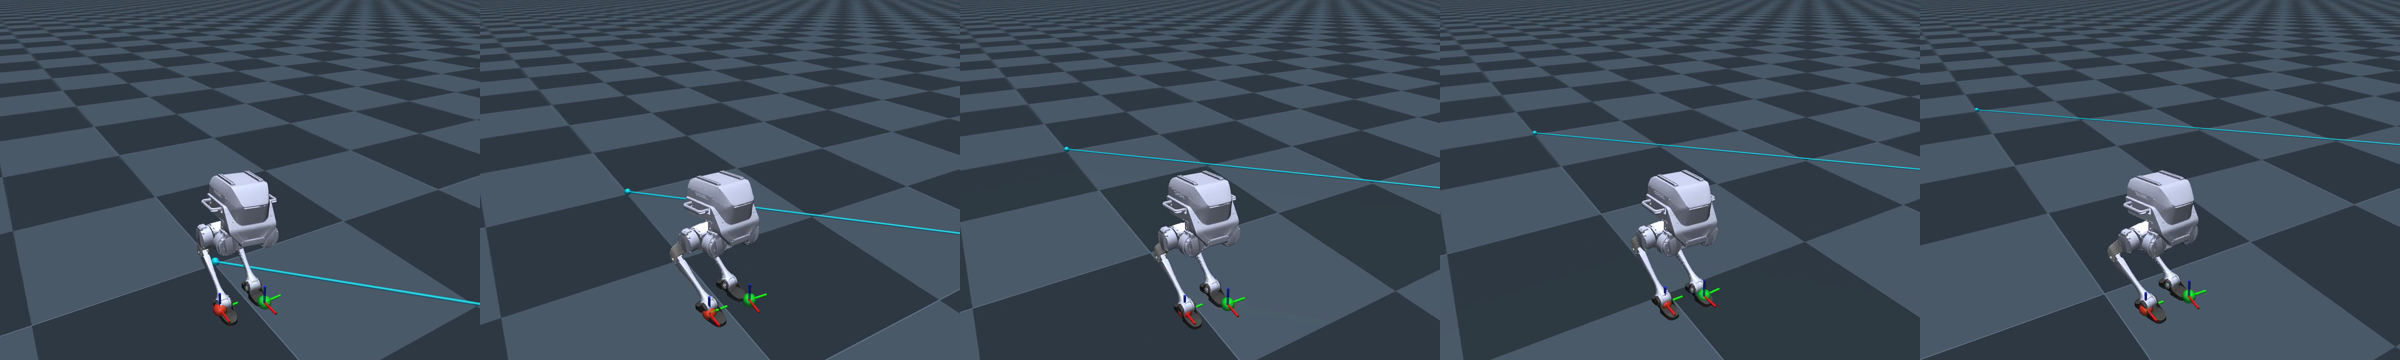
\includegraphics[width=\linewidth]{assets/lower_sequence.png}
\centering\videotext{lower_foothold_50s.mp4}{点击播放 50 s 下层执行视频}
\column{0.42\textwidth}
\small
\begin{tabular}{lr}
\toprule
指标 & 结果\\
\midrule
连续时长 & 50 s\\
触地次数 & 99\\
触地 $xy$ 误差均值 & 2.65 cm\\
P95 & 4.91 cm\\
最大值 & 5.78 cm\\
$<10$ cm 比例 & 100\%\\
低高度/大倾角信号 & 0\\
\bottomrule
\end{tabular}
\vspace{0.5em}
接口扫描：27/27 个确定性目标未跌倒，23/27 的触地 P95 小于 5 cm。随机重复 108 组均未跌倒，但每个 seed 仅约 11--12/27 达到 P95 小于 5 cm。
\end{columns}
\vspace{0.3em}
结论限于当前证据：下层已能稳定执行平面落足目标，但精确度受随机性影响，且尚未建立非零高度脚目标能力。
\end{frame}

\begin{frame}{单中心障碍：视觉闭环产生明确绕行行为}
\begin{columns}[T,onlytextwidth]
\column{0.52\textwidth}
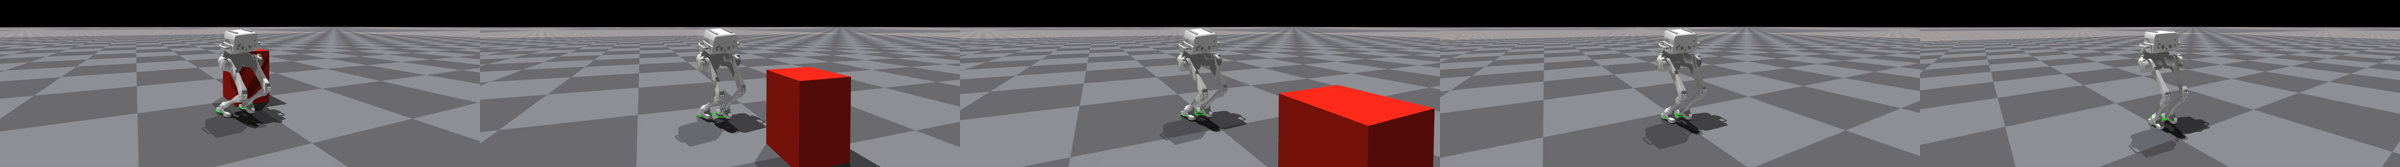
\includegraphics[width=\linewidth]{assets/single_obstacle_30s.png}
\centering\videotext{single_obstacle_30s.mp4}{点击播放 30 s 对照视频}
\column{0.45\textwidth}
\small
16 个并行环境，30 s，seed 307：
\begin{tabular}{lrrr}
\toprule
策略 & 完成 & 碰撞 & 物理终止\\
\midrule
中性落足 & 0 & 585 & 123\\
视觉 CEM & 14 & 204 & 33\\
深度打乱 & 7 & 270 & 51\\
深度置零 & 0 & 761 & 19\\
\bottomrule
\end{tabular}
\vspace{0.5em}
视觉 CEM 的平均前进量为 1.92 m，中性落足为 0.33 m。深度打乱后性能居中、置零后完成归零，说明结果不只来自固定方向脚印。
\end{columns}
\vspace{0.3em}
表中“完成”为自动 reset 前累计完成事件，不等同于独立 episode 成功率。
\end{frame}

\begin{frame}{三障碍：五步真实序列训练的阶段效果}
\begin{columns}[T,onlytextwidth]
\column{0.52\textwidth}
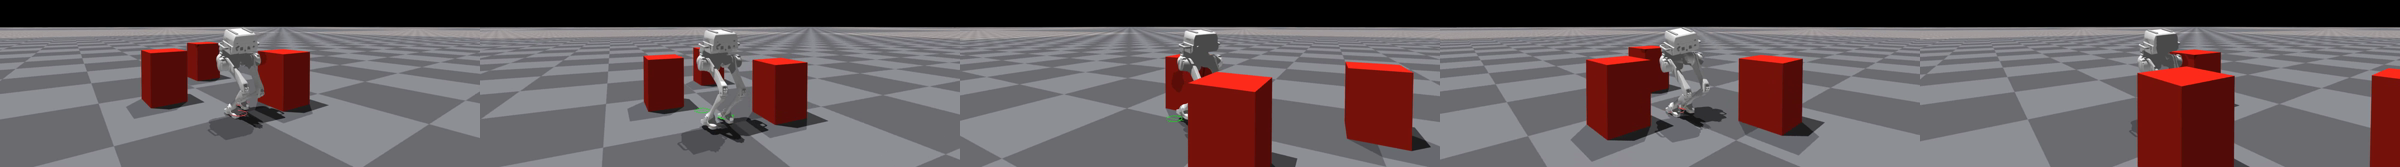
\includegraphics[width=\linewidth]{assets/three_obstacles_30s.png}
\centering\videotext{three_obstacles_30s.mp4}{点击播放 30 s 三障碍视频}
\column{0.45\textwidth}
\small
16 个并行环境，30 s，seed 318：
\begin{tabular}{lrrr}
\toprule
模型 & 完成 & 碰撞 & 物理终止\\
\midrule
课程 1 基线 & 2 & 381 & 14\\
one-step 训练 & 2 & 261 & 33\\
5-step 训练 & 5 & 137 & 16\\
\bottomrule
\end{tabular}
\vspace{0.5em}
相对 one-step，五步训练的碰撞事件由 261 降至 137，同时完成事件由 2 增至 5；说明按真实换脚连续序列训练，对多障碍下的规划有效。
\end{columns}
\vspace{0.3em}
当前完成计数仍低，此结果主要用于验证“多步宏观模型”实现逻辑，而非证明复杂场景已解决。
\end{frame}

\begin{frame}{窄桥：落足规划对狭窄支撑区域的效果}
\begin{columns}[T,onlytextwidth]
\column{0.52\textwidth}
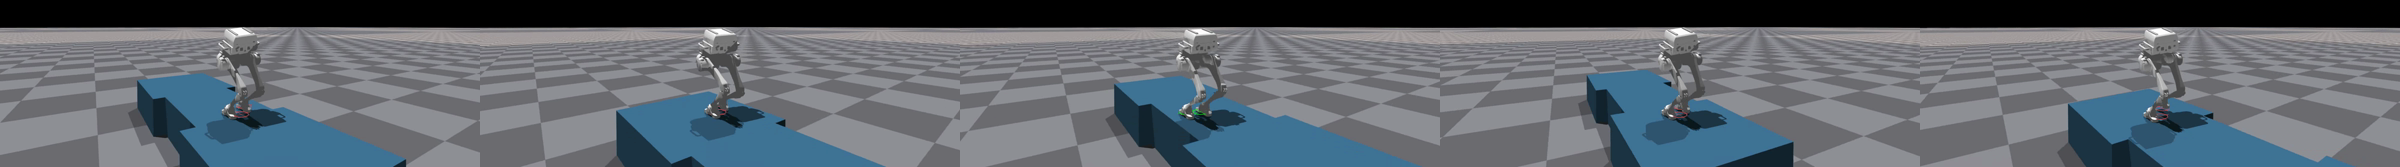
\includegraphics[width=\linewidth]{assets/narrow_bridge_planner_20s.png}
\centering\videotext{narrow_bridge_planner_20s.mp4}{点击播放 20 s 规划器视频}
\column{0.45\textwidth}
\small
12 个并行环境，20 s，seed 426；桥宽 0.75--0.95 m，课程长度 2.5 m：
\begin{tabular}{lrrrr}
\toprule
策略 & 完成 & 碰撞 & 终止 & 越界\\
\midrule
中性落足 & 18 & 0 & 4 & 6\\
视觉规划 & 30 & 1 & 1 & 3\\
\bottomrule
\end{tabular}
\vspace{0.5em}
规划器以一次额外碰撞为代价，将完成事件从 18 增至 30，物理终止从 4 降至 1，越界从 6 降至 3。
\end{columns}
\vspace{0.3em}
这是当前最直接体现“视觉选择落足位置—下层闭环执行—显式支撑区域标签”组合效果的小场景。
\end{frame}

\begin{frame}{典型地形结果：可运行案例与当前失败模式}
\begin{columns}[T,onlytextwidth]
\column{0.51\textwidth}
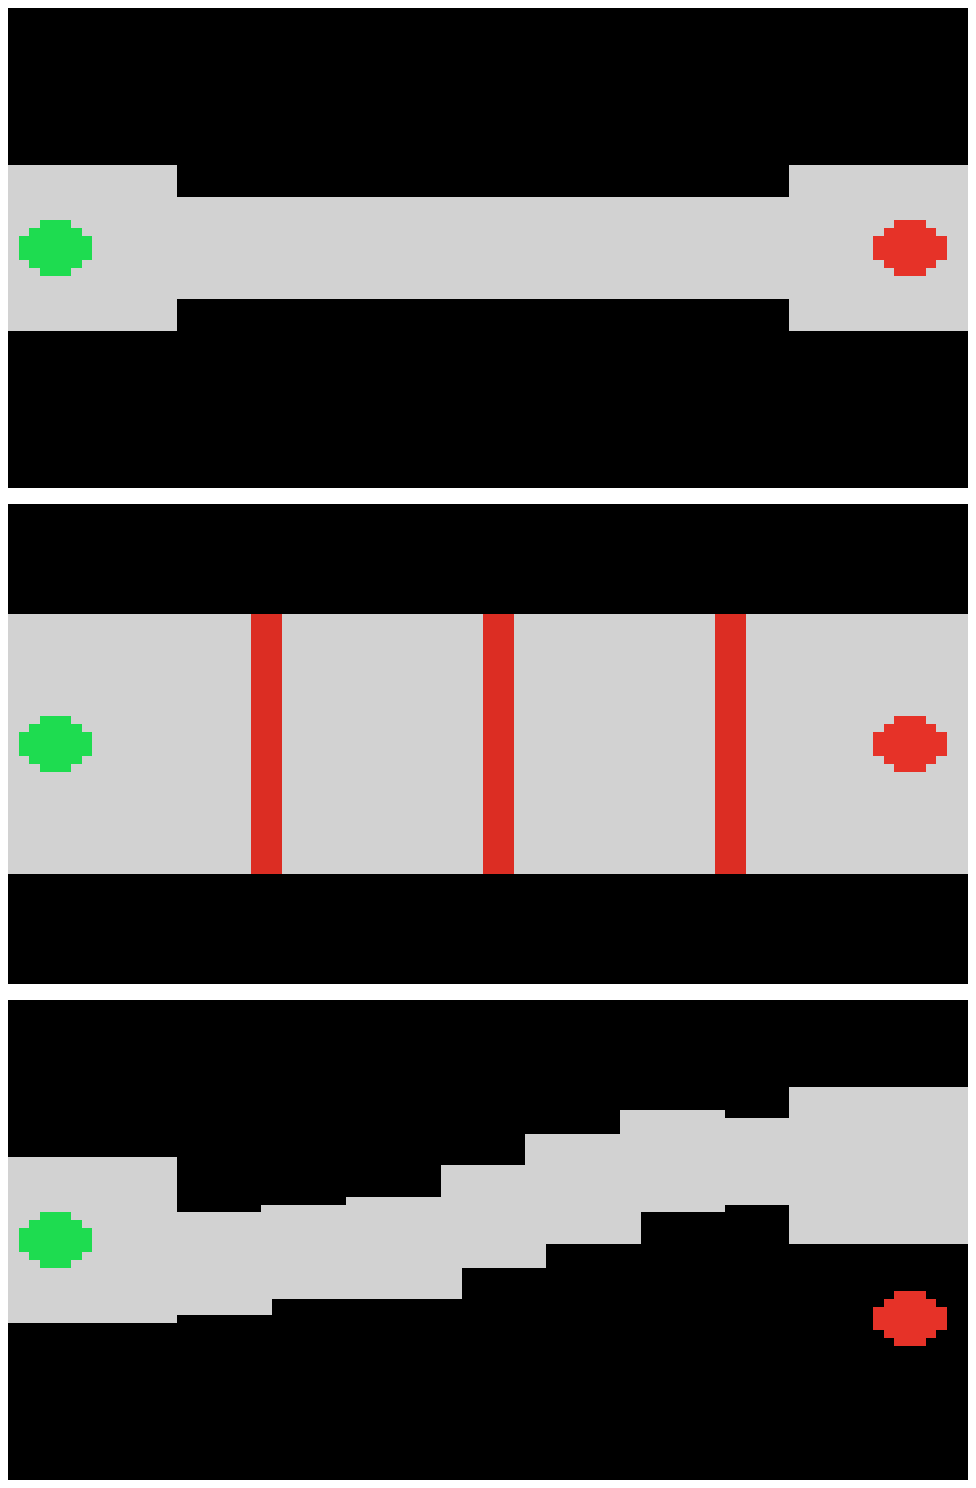
\includegraphics[width=\linewidth,height=0.58\textheight,keepaspectratio]{assets/typical_terrain_montage.png}
\column{0.46\textwidth}
\small
12 个并行环境，30 s，seed 422：
\begin{tabular}{lrrrr}
\toprule
版本 & 完成 & 终止 & 碰撞 & 越界\\
\midrule
旧模型 & 0 & 5 & 6 & 9\\
mixed & 1 & 33 & 28 & 27\\
加越界监督 & 3 & 27 & 43 & 20\\
\bottomrule
\end{tabular}
\vspace{0.4em}
\videotext{narrow_bridge_neutral_5s.mp4}{窄桥中性落足 5 s}\par
\videotext{hurdles_neutral_5s.mp4}{低障碍运行 5 s}\par
\videotext{irregular_support_failure_5s.mp4}{不规则支撑失败 5 s}
\end{columns}
\vspace{0.3em}
当前模型能在典型地形中运行并产生非中性落足选择，但 mixed 场景的完成仍少、终止与碰撞较多；不规则支撑面和高度变化是最明显的失败来源。
\end{frame}

\begin{frame}{结果汇总：目前能由实验直接支持的结论}
\small
\begin{tabular}{p{0.24\textwidth}p{0.34\textwidth}p{0.34\textwidth}}
\toprule
模块/问题 & 已有正向证据 & 当前边界\\
\midrule
下层目标执行 & 50 s 99 次触地，P95 4.91 cm，无跌倒信号 & 随机扫描的 5 cm 精度不稳定；仅平面目标\\
视觉是否被使用 & 单障碍视觉 CEM 优于中性、打乱和置零深度 & 单 seed，尚未形成统计置信区间\\
多步模型是否有效 & 三障碍 5-step 相对 one-step 降碰撞、增完成 & 绝对完成数仍低\\
狭窄支撑区 & 窄桥中规划器增完成、降终止和越界 & 桥宽与动作范围经过课程化限制\\
通用复杂地形 & 已能启动训练、执行、记录事件与视频 & 不规则支撑和高度变化尚未可靠解决\\
\bottomrule
\end{tabular}
\vspace{0.7em}
因此，当前阶段可以确认的是：\textbf{分层接口、宏观数据闭环、五步世界模型训练与 CEM 在线控制均已实现，并在若干小场景中产生可观察优势。}
\end{frame}

\begin{frame}{可采用的方法提案：复杂地形快速泛化}
\small
\begin{block}{任务定义}
训练时组合平地、窄桥、低障碍、稀疏支撑和有限高度变化；测试时更换地形布局、尺寸与组合顺序。上层只重规划落足，冻结下层保持相同关节控制接口。
\end{block}
\begin{block}{方法形式}
\begin{itemize}
  \item 输入保持 $(D_k,p_k,g_k)$，动作保持 $(\rho_k,\theta_k,\psi_k)$；
  \item 支撑区域标签监督 $I^{off}$，碰撞/跌倒头监督接触风险；
  \item 若加入高度动作，可将上层扩展为 $u_k=(\rho,\theta,\Delta z,\psi)$，同时重新训练下层的非零高度目标分布；
  \item 评价以新地形成功率、碰撞/越界次数、触地误差和少量微调后的恢复速度为主。
\end{itemize}
\end{block}
该提案直接对应当前已实现结构；新增的关键能力是非零 $\Delta z$ 落足，而不是增加新的规划层或独立地图模块。
\end{frame}

\begin{frame}{可采用的方法提案：家庭空间低碰撞狭窄到达}
\small
\begin{block}{任务定义}
机器人从房间随机初始位姿出发，在桌椅、沙发、墙角等静态障碍间到达指定站位；目标区域允许转身但通道和最终站位较窄，统计全身非足碰撞。
\end{block}
\begin{block}{与当前框架的对应关系}
\begin{itemize}
  \item 深度图提供局部障碍几何；相对目标提供导航方向；
  \item 上层在 0.5 s 时间尺度选择步长、横向落足和脚朝向，可在狭窄区域主动缩步、侧步或转脚；
  \item 下层维持动态平衡并吸收单步执行误差；事件头直接预测全身碰撞和跌倒风险；
  \item 新房间可先零样本使用已有模型，再用少量宏观 transition 更新世界模型，而无需重训高频关节策略。
\end{itemize}
\end{block}
可能体现的优势是：相较纯几何局部避障，规划代价来自完整机器人经闭环步行后的真实碰撞；相较端到端关节策略，迁移时主要更新低频世界模型，数据单位是一次落足而非每个物理步。
\end{frame}

\begin{frame}{最小后续验证范围}
\small
\begin{tabular}{p{0.23\textwidth}p{0.31\textwidth}p{0.37\textwidth}}
\toprule
目的 & 最小实验设置 & 需要报告的指标\\
\midrule
确认下层动作域 & 前/后/侧向及偏航目标网格，多随机 seed & 跌倒率、触地均值/P95/最大误差\\
确认视觉闭环 & 单障碍与窄桥，各使用固定测试 seed 集合 & episode 成功率、每米碰撞、终止、越界\\
确认多步训练作用 & one-step 与 5-step，只改变序列损失 & 同一场景同一预算下的上述指标\\
确认新场景迁移 & 未见布局：零样本及少量 transition 更新 & 成功率随数据量变化、碰撞与微调时间\\
\bottomrule
\end{tabular}
\vspace{0.8em}
对比范围保持最小：中性/规则落足、当前 one-step 版本、当前 5-step 完整模型。其余外部方法只有在场景和评价口径稳定后再选择一到两个代表性基线。
\end{frame}

\begin{frame}{视频与文件索引}
\small
\begin{tabular}{p{0.37\textwidth}p{0.53\textwidth}}
\toprule
文件 & 内容\\
\midrule
\videotext{lower_foothold_50s.mp4}{lower\_foothold\_50s.mp4} & 下层连续目标落足，50 s\\
\videotext{single_obstacle_30s.mp4}{single\_obstacle\_30s.mp4} & 单中心障碍视觉闭环对照，30 s\\
\videotext{three_obstacles_30s.mp4}{three\_obstacles\_30s.mp4} & 三障碍五步规划，30 s\\
\videotext{narrow_bridge_planner_20s.mp4}{narrow\_bridge\_planner\_20s.mp4} & 窄桥视觉规划器，20 s\\
\videotext{narrow_bridge_neutral_5s.mp4}{narrow\_bridge\_neutral\_5s.mp4} & 窄桥中性落足，5 s\\
\videotext{hurdles_neutral_5s.mp4}{hurdles\_neutral\_5s.mp4} & 低障碍运行，5 s\\
\videotext{irregular_support_failure_5s.mp4}{irregular\_support\_failure\_5s.mp4} & 不规则支撑失败案例，5 s\\
\bottomrule
\end{tabular}
\vspace{0.7em}
所有视频位于 PDF 同级目录的 \code{media/} 文件夹。部分 PDF 阅读器会禁用 \code{run:} 链接，此时可直接打开相应文件。
\end{frame}

\begin{frame}{总结}
\begin{enumerate}
  \item 下层将双脚目标位姿、步态相位和本体状态编码为 46 维 Actor 输入，以 50 Hz 生成 8 维关节位置增量；通过目标采样、落足跟踪和稳定性奖励训练得到可冻结的闭环落足执行器。
  \item 上层在真实换脚处读取 $64\times64$ 深度和 36 维本体状态，输出三维支撑脚相对落足动作；五步潜空间模型预测进度、奖励、价值和风险事件，CEM 每 0.5 s 重规划。
  \item 工程上已打通目标解码、闭环执行、宏观事件聚合、连续 replay、五步模型训练、在线规划、评估和视频记录。
  \item 当前结果支持该方法在单障碍、三障碍和窄桥小场景中的可行性；复杂高度地形和跨家庭空间泛化仍属于待验证的方法提案。
\end{enumerate}
\end{frame}

\end{document}
